\documentclass[pdftex]{article}
% \documentclass[prl,showpacs,amsmath,amssymb]{revtex4} % PRL

% margins of 1 inch:
\setlength{\topmargin}{-.5in}
\setlength{\textheight}{9in}
\setlength{\oddsidemargin}{0in}
\setlength{\textwidth}{6.5in}

\usepackage[pdftex]{hyperref} % hyperlink equation and bibliographic citations
\usepackage[dvips]{graphicx,color}
\usepackage{amsmath} % advanced math
\usepackage{verbatim} % multi-line comments
\usepackage{natbib} % bibilography
\usepackage{mciteplus} % collapse multiple citations in bibilography

% from http://www.flakery.org/search/show/569

\newcommand{\infint}{\ensuremath{\int_{-\infty}^{\infty}}}

\newcommand{\ie}{\textit{i.e.}\ }
\newcommand{\eg}{\textit{e.g.}\ }

\newcommand{\eqn}[1]{Eq.\ (\ref{#1})}

\newcommand{\pfrac}[2]{\ensuremath{\frac{\partial #1}{\partial #2}}}

\begin{document}

\title{Network Model}

\author{Ben Payne$^{1}$\footnote{Electronic address: bpayne@lps.umd.edu}
{\it $^{1}$Department of Fun, University Name \& Town, city, State Zip}}

\date{\today}

% \begin{abstract}
% Model random networks
% \end{abstract}

%\maketitle % declares end of title page

\tableofcontents

%\newpage

\section{Introduction}

There are two methods to model a network:
\begin{itemize}
 \item create a database of port connections
 \item create autonomous switches which direct packets to other components
\end{itemize}
For this model I will be using a database of connections.

\subsection{problem}

We want an all-to-all network. 

An optimal all-to-all design would have each compute node with $N-1$ ports and no switches (0 hops).
\begin{figure}[h!]
\begin{center}
(a)\ \includegraphics[scale=0.2]{pictures/N2_n1_M0_mNA}\ \ \ 
(b)\includegraphics[scale=0.2]{pictures/N3_n1_M0_mNA}\ \ \ 
(c)\ \includegraphics[scale=0.2]{pictures/N4_n1_M0_mNA}\ \ \ 
(d)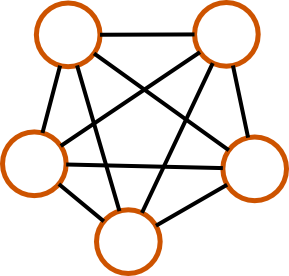
\includegraphics[scale=0.2]{pictures/N5_n1_M0_mNA}\\*
\caption{increasing the number of nodes. Doesn't scale well due to limited number of ports on each compute node ($n<N$).}
\end{center}
\end{figure}
For $N>1000$ this simplisitic approach is not feasiable. Thus we introduce switches.
\begin{figure}[h!]
\begin{center}
(a)\includegraphics[scale=0.2]{pictures/N4_n1_M1_m4}\ \ \ 
(b)\includegraphics[scale=0.2]{pictures/N6_n1_M2_m4}\\*
\caption{adding switches. Doesn't scale well due to limited number of ports per switch ($m<N$). Also, conjestion (a,b) and bisection bandwidth (a) are poor.}
\end{center}
\end{figure}

To reduce conjestion and increase bisection bandwidth, add more switches. Also increase the number of ports per compute node. Then the optimization problem becomse non-trivial.

\subsection{objectives}

If I can show a given topology is better than some other, that is useful.

If I can show how one switch versus another (differentiated by number of ports) affects performance, that is useful.

\subsection{Does Topology matter? A toy model example}

Suppose now we have $N=5$ compute nodes with 1 port each. Then the optimal network design (fewest hops) is to have a 5 port switch:
\begin{figure}[h!]
\begin{center}
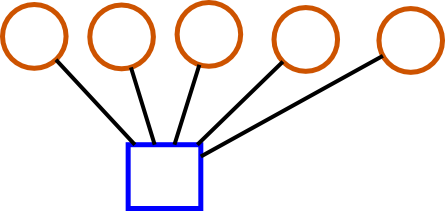
\includegraphics[scale=0.2]{pictures/N5_n1_M1_m5.png}\\*
\caption{Here number of hops is 1 for each compute node, with 10 pairs (=5*4/2).}
\end{center}
\end{figure}

The other extreme would be to use five of these same switches with only one compute node per switch:
\begin{figure}[h!]
\begin{center}
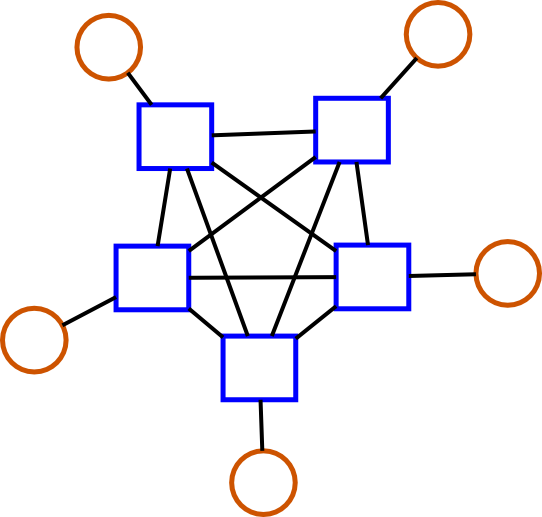
\includegraphics[scale=0.2]{pictures/N5_n1_M5_m5.png}\\*
\caption{Here number of hops is 2 for each compute node.}
\end{center}
\end{figure}
Clearly we are spending too much money on switches for the same number of compute nodes. However, this increased hop count (2) also lowers conjestion.

As a compromise, we can use two switches and increase the number of compute nodes:

\begin{figure}[h!]
\begin{center}
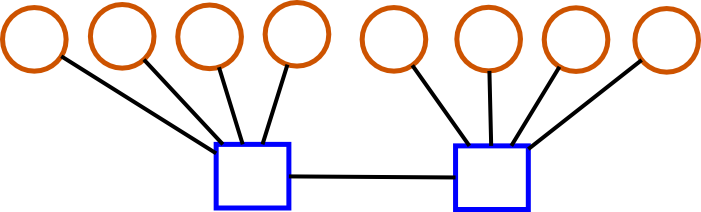
\includegraphics[scale=0.2]{pictures/N8_n1_M2_m5.png}\\*
\caption{8 nodes and 2 switches: 12 pairs with 1 hop, 16 pairs with 2 hops.}
\end{center}
\end{figure}

\begin{figure}[h!]
\begin{center}
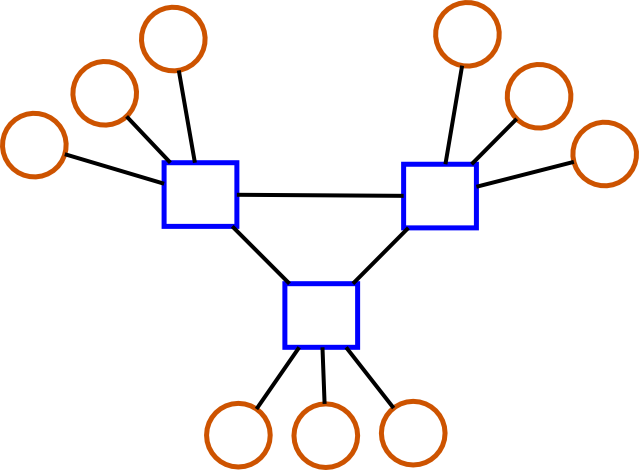
\includegraphics[scale=0.2]{pictures/N9_n1_M4_m5.png}\\*
\caption{1 or 2 hops, 9 nodes and 3 switches.}
\end{center}
\end{figure}
Notice a few constraints were followed:
\begin{itemize}
 \item each switch has same number of ports
 \item each compute node has one port
 \item each switch is fully occupied
 \item each node can reach every other node
 \item each switch has at least one computer connected to it
\end{itemize}

The number of permutations increases when we have more than 9 compute nodes and only 5 ports. Even worse, consider when there are multiple ports per computer (but much less than the number of computers).

The parameter space includes
\begin{itemize}
 \item number of computers
 \item number of ports per computer
 \item number of switches
 \item number of ports per switch
\end{itemize}
Metrics:
\begin{itemize}
 \item hop count for each pair\\
 How to measure hop count for all pairs:
\begin{itemize}
 \item \href{http://en.wikipedia.org/wiki/Floyd\%E2\%80\%93Warshall_algorithm}{http://en.wikipedia.org/wiki/Floyd\%E2\%80\%93Warshall\_algorithm}
 \item \href{http://www.cs.rochester.edu/u/nelson/courses/csc_173/graphs/apsp.html}{http://www.cs.rochester.edu/u/nelson/courses/csc\_173/graphs/apsp.html}
 \item \href{http://stackoverflow.com/questions/5249857/all-pairs-all-paths-on-a-graph}{http://stackoverflow.com/questions/5249857/all-pairs-all-paths-on-a-graph}
\end{itemize}
Might be able to get away with finding average hop count and maximum hop count if (1) that is all we care about and (2) there's a faster algorithm for those counts.
%  \begin{itemize}
%   \item average hop count
%   \item maximum hop count
%  \end{itemize}
 \item bisection bandwidth\\
 How to measure bisection bandwidth: chose a random set of half the switches. Move these to one side and determine how many cuts need to be made to separate the two halves.
\end{itemize}


\subsection{Permutations}

The number of unique pairs on a network swith $N$ computers is $N(N-1)/2$. 

When $N=4$ then there are 6 pairs. $N=100$ is 4950 pairs. $N=10,000$ is 49,995,000 pairs.

\section{standard networks}

See \href{http://www.cs.nmsu.edu/~pfeiffer/classes/573/notes/topology.html}{http://www.cs.nmsu.edu/~pfeiffer/classes/573/notes/topology.html}

\subsection{Mesh}
Mesh (and the related torus) can be of $n$ dimensions, commonly $n=$2, 3, 6. Useful for physical sciences due to local communication (nearest neighbors).
\begin{comment}
##Command to produce the output: "neato -Tpng thisfile.gv > thisfile.png"
##Command to produce the output: "circo -Tpng thisfile.gv > thisfile.png"
graph G {
node [shape=box,color=red,style=bold];  c0;
node [shape=box,color=red,style=bold];  c1;
node [shape=box,color=red,style=bold];  c2;
node [shape=box,color=red,style=bold];  c3;
node [shape=box,color=red,style=bold];  c4;
node [shape=box,color=red,style=bold];  c5;
node [shape=box,color=red,style=bold];  c6;
node [shape=box,color=red,style=bold];  c7;
node [shape=box,color=red,style=bold];  c8;
node [shape=circle,fixedsize=true,width=0.9,color=blue,style=bold];  s0;
node [shape=circle,fixedsize=true,width=0.9,color=blue,style=bold];  s1;
node [shape=circle,fixedsize=true,width=0.9,color=blue,style=bold];  s2;
node [shape=circle,fixedsize=true,width=0.9,color=blue,style=bold];  s3;
node [shape=circle,fixedsize=true,width=0.9,color=blue,style=bold];  s4;
node [shape=circle,fixedsize=true,width=0.9,color=blue,style=bold];  s5;
node [shape=circle,fixedsize=true,width=0.9,color=blue,style=bold];  s6;
node [shape=circle,fixedsize=true,width=0.9,color=blue,style=bold];  s7;
node [shape=circle,fixedsize=true,width=0.9,color=blue,style=bold];  s8;
     s0--c0;
     s1--c1;
     s2--c2;
     s3--c3;
     s4--c4;
     s5--c5;
     s6--c6;
     s7--c7;
     s8--c8;
     s0--s1; 
     s0--s3;
     s1--s2;
     s1--s4;
     s2--s5;
     s3--s4;
     s3--s6;
     s4--s7;
     s4--s5;
     s5--s8;
     s6--s7;
     s7--s8;
     overlap=false
     label="3x3 mesh\nlayed out by Graphviz"
     fontsize=12;
}
\end{comment}
Mesh networks are well-characterized. ``Meshes have O(n) cost, O(sqrt(n)) bisection bandwidth, O(n) aggregate bandwidth, and O(sqrt(n)) latency.''

\begin{figure}[h!]
\begin{center}
 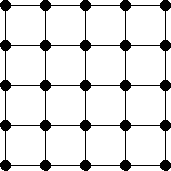
\includegraphics[scale=.5]{pictures/mesh}
\end{center}
\end{figure}



\subsection{Hypercube}

``the latency is is O(log N). There are N processors, each with log2N interfaces, so the cost is O(N log N). and all the processors can use their links simultaneously, so our aggregate bandwidth is O(N). The bisection bandwidth is O(log N).''

\subsection{Fat Tree}

\href{http://en.wikipedia.org/wiki/Fat_tree}{http://en.wikipedia.org/wiki/Fat\_tree}

\subsection{Flattened Butterfly}

\subsection{Dragonfly}

\href{http://research.google.com/pubs/pub34926.html}{http://research.google.com/pubs/pub34926.html}

Fractal

\subsection{Clos Network}

\href{http://en.wikipedia.org/wiki/Clos_network}{http://en.wikipedia.org/wiki/Clos\_network}

\subsection{randomly-connected networks}

For networks supporting physical models (i.e., mesh), it makes sense to think about dimension, perimeter/surface area, area/volume. This may not apply to scale-free topologies. 

If the topology turns out to be scale free, then we wouldn't need to model 1E6 endpoints (that is desirable).

\section{more than one port per endpoint}

If each endpoint has only one network connection, then we can model a switch-only network. A switch with 4 ports not connected to other switches would have 4 endpoints.

\section{random network creation}

For a given \{(number of computers), (number of ports per computer), (number of ports per switch)\}, should random computers be plugged into random port switches, or should random switches be connected first?

\ \\
``connections'' database methods:
\begin{itemize}
 \item each switch is an sub-array of the connections array. The elements of each sub-array denote which computer the switch is plugged into. 
 \item connections pairs: computer--switch and switch-switch. The connections array has sub-arrays of size 2 for each edge of the graph (nodes are either computers or switches).
 \begin{itemize}
  \item unordered pairs of positive (switch) and negative (computer) integer indices
 \end{itemize}

\end{itemize}
Features needed:
 \begin{itemize}
  \item supports switches having arbitrary port count (not all switches must have same number of ports
 \end{itemize}


\ \\
Whether local symmetry (same number of computers plugged into each switch) is a hinderance, benefit, or irrelevant is not clear to me.

Random connections lead to unexpected paths. This could be good, bad, or inconsequential.

\section{route enumeration}

\begin{enumerate}
 \item For each computer, see what other computers are available on the same switch (1 hop)
 \item For each computer, see what other computers are two switches away (2 hops)
 \item ...
\end{enumerate}
When a switch has had all of its computers touched for a given iteration, then we should mark that switch as ``touched'' (doesn't need to be queried again for current iteration). That is, mark a switch to indicate ``all locally-attached computers have number of hops known.'' This should reduce search time.

\section{Maximum and Minimum number switches needed}
How many switches ($M$) are needed when each switch has $m$ ports? (Assume $m<(N-1)$.)

Variables: 
\begin{itemize}
 \item $n$ = number ports per compute node
 \item $N$ = number of compute nodes
\item $m$ = number of ports per switch
 \item $M$ = number of switches
\end{itemize}
Observe that we have already made the simplifying assumption of identical compute nodes and identical switches.

\subsection{one port per compute node}
For $N$ compute nodes, how many switches $M$ are needed when each switch has $m$ ports? We assume there are more compute nodes than ports on one switch ($m<(N-1)$). We must obey the constraints (every compute node must be able to reach every other compute node -- ``fully connected network''), (all switch ports are used), (all compute node ports are used).

\textbf{Solution 1}: to get an all-to-all network, each node should connect to a tree with $(N-1)$ endpoints (bisection bandwidth is thus maximized). To acheive this, start with one compute node and a switch with $m$ ports (for this example let $m=5$). At this tree level ($k=1$) we have $m=5$, $M'=1$, and $N-1=4$. ($M'$ refers to the number of switches for this one compute node).

\begin{figure}[h!]
\begin{center}
\includegraphics[scale=0.3]{pictures/N5_n1_M1_m5_tree}
\label{fig:tree_k1}
 \caption{$m=5$, $M'=1$, $N-1=4$ (tree level $k=1$). }
\end{center}
\end{figure}

\begin{figure}[h!]
\begin{center}
\includegraphics[scale=0.3]{pictures/N17_n1_M5_m5_tree}
\label{fig:tree_k2}
 \caption{$m=5$, $M'=1+4$, $N-1=4*4$ (tree level $k=2$). }
\end{center}
\end{figure}


\begin{figure}[h!]
\begin{center}
\includegraphics[scale=0.3]{pictures/N65_n1_M21_m5_tree}
\label{fig:tree_k3}
 \caption{$m=5$, $M'=1+4+4^2$, $N-1=4^3$ (tree level $k=3$). }
\end{center}
\end{figure}

Generalizing, the number of compute nodes the one we are dealing with can connect to is
\begin{equation}
 N-1=(m-1)^k
 \label{eq:Nminus1k}
\end{equation}
and the number switches this one compute node needs to create $N-1$ endpoints is
\begin{equation}
 M'=\sum_{a=1}^{k} (m-1)^{(a-1)}
\end{equation}
Since there are a total of $N$ compute nodes, the total number of switches $M$ needed is
\begin{equation}
\boxed{
 M_{max}=N\sum_{a=1}^{k} (m-1)^{(a-1)}
 }
\end{equation}
This is the maximum number of switches needed.

We can solve for $k$ from Eq.~\ref{eq:Nminus1k}
\begin{equation}
 \log(N-1)=k\log(m-1)
\end{equation}
\begin{equation}
 k=\frac{\log(N-1)}{\log(m-1)}
 \label{eq:k_n1}
\end{equation}
valid values: $m>2$ and $N>2$.

For Matlab/Octave,
\begin{verbatim}
 a=1:ceil(log(N-1)/log(m-1)); M_max=N*sum((m-1).^(a-1))
\end{verbatim}
Note: use of ``ceil'' gives worse case scenario in which there are empty switch ports. This equation is accurate when Eq.~\ref{eq:k_n1} is an integer (then ``ceil'' is not used).

\textbf{Solution 2}: the minimum number of switches needed can be found by daisy-chaining switches together. We can enumerate this by seeing how many compute nodes can be attached to 1 switch, then 2 switches, and so on. 

\begin{figure}[h!]
\begin{center}
\includegraphics[scale=0.3]{pictures/N5_n1_M1_m5}
\label{fig:neq15}
 \caption{$m=5$, $M=1$, $N=5$}
\end{center}
\end{figure}

\begin{figure}[h!]
\begin{center}
\includegraphics[scale=0.3]{pictures/N8_n1_M2_m5}
\label{fig:neq18}
 \caption{$m=5$, $M=2$, $N=4+4=8$}
\end{center}
\end{figure}

\begin{figure}[h!]
\begin{center}
\includegraphics[scale=0.3]{pictures/N11_n1_M3_m5}
\label{fig:neq111}
 \caption{$m=5$, $M=3$, $N=4+3+4$}
\end{center}
\end{figure}

\begin{figure}[h!]
\begin{center}
\includegraphics[scale=0.3]{pictures/N14_n1_M4_m5}
\label{fig:neq114}
 \caption{$m=5$, $M=4$, $N=4+3+3+4$}
\end{center}
\end{figure}

Thus, for $M>1$, 
\begin{equation}
 N=(m-1)+(M-2)(m-2)+(m-1)=2(m-1)+(M-2)(m-2)
\end{equation}
This solution has a high hop count and low bisection bandwidth of 1.

Solving for $M$,
\begin{equation}
\boxed{
M_{min}= \frac{N-2(m-1)}{m-2}+2
}
\label{eq:maximum_neq1}
\end{equation}
where $m>2$ and $N>2(m-1)$.

For Matlab/Octave,
\begin{verbatim}
M_min=(N-(2*(m-1)))/(m-2)+2 
\end{verbatim}


\ \\
As an example, when $N=1000$ and $m=24$, the maximum number of switches is 553,000 (solution 1) and the minimum is 46 (solution 2).

\subsection{more than one port per compute node}
What is the maximum switch count when there are two ports per compute node ($n=2$)? 

\textbf{Solution 1} (maximum number of switches): Start with one compute node and a switch with $m$ ports (for this example let $m=5$). At this tree level ($k=1$) we have $m=5$, $M'=2$, and $N-1=2*4=8$. ($M'$ refers to the number of switches for this one compute node).


\begin{figure}[h!]
\begin{center}
\includegraphics[scale=0.3]{pictures/N9_n2_M2_m5_tree}
\label{fig:ngt1k1}
 \caption{$m=5$, $M'=2$, $N-1=2*4$ (tree level $k=1$). }
\end{center}
\end{figure}

\begin{figure}[h!]
\begin{center}
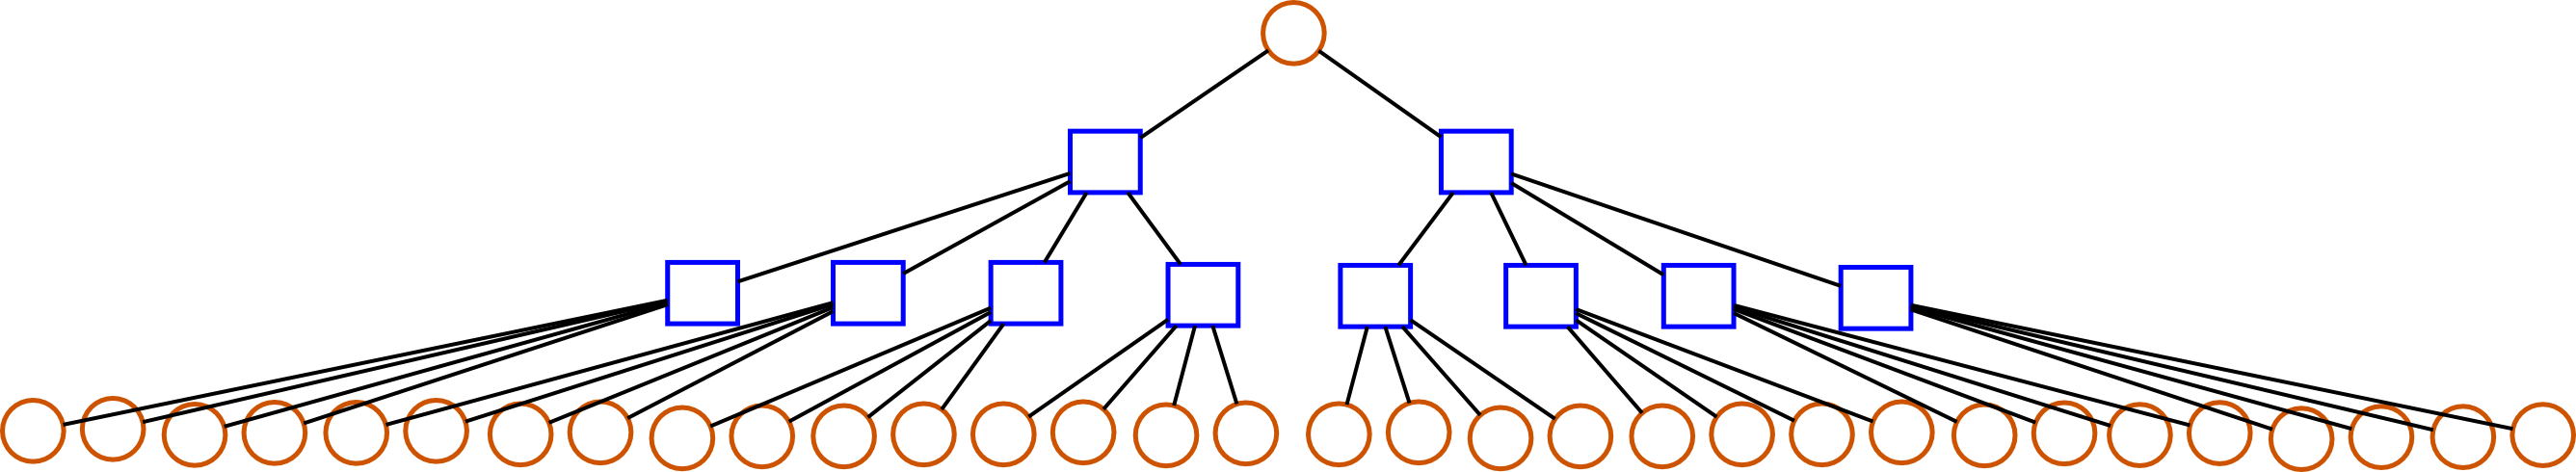
\includegraphics[scale=0.3]{pictures/N33_n2_M10_m5_tree}
\label{fig:ngt1k2}
 \caption{$m=5$, $M'=2+2*4$, $N-1=2*4*4$ (tree level $k=2$). }
\end{center}
\end{figure}

% \begin{figure}[h!]
% \begin{center}
% \includegraphics[scale=0.3]{pictures/}
% \label{fig:ngt1k2}
%  \caption{$m=5$, $M'=2+2*4$, $N-1=2*4*4$ (tree level $k=2$). }
% \end{center}
% \end{figure}


% \begin{figure}[h!]
% \begin{center}
% \includegraphics[scale=0.3]{pictures/}
% \label{fig:ngt1k3}
%  \caption{$m=5$, $M'=2+2*4+4^2$, $N-1=2*4^3$ (tree level $k=3$). }
% \end{center}
% \end{figure}

Generalizing, the number of nodes this one can connect to is
\begin{equation}
 N=n(m-1)^k
 \label{eq:Nminus1kngt1}
\end{equation}
and the number of switches for this one compute node is
\begin{equation}
 M'=n\sum_{a=1}^{k} (m-1)^{(a-1)}
\end{equation}
As before, the total number of switches needed is $M=N M'$,
\begin{equation}
\boxed{
 M_{max}=N n\sum_{a=1}^{k} (m-1)^{(a-1)}
 }
 \label{eq:maximum_ngt1}
\end{equation}
and we can solve Eq.~\ref{eq:Nminus1kngt1} to find $k$
\begin{equation}
 \log(N-1)=\log(n) + k\log(m-1)
\end{equation}
\begin{equation}
 k=\frac{\log((N-1)/n)}{\log(m-1)}
 \label{eq:k_many_n}
\end{equation}

For Matlab/Octave,
\begin{verbatim}
a=1:ceil(log((N-1)/n)/log(m-1)); M_max=N*n*sum((m-1).^(a-1))
\end{verbatim}
Note: use of ``ceil'' gives worse case scenario in which there are empty switch ports. This equation is accurate when Eq.~\ref{eq:k_many_n} is an integer (then ``ceil'' is not used).

The maximum number of switches as given by Eq.~\ref{eq:maximum_ngt1} is expected to be less than the value from Eq.~\ref{eq:maximum_neq1} since there are more ports supplied at the compute node.

\textbf{Solution 2} (minimum number of switches): Again we will start with $n=2$ and find how many compute nodes are supported with 1 switch, then 2 switches, and so on. Here we will assume $m=4$. We cannot use one switch for two compute nodes because it violates our earlier assumption that no compute node should connect to the same switch twice.

With two switches, we can connect 4 compute nodes.

\begin{figure}[h!]
\begin{center}
\includegraphics[scale=0.3]{pictures/N4_n2_M2_m4}
\label{fig:ngt14}
 \caption{$m=4$, $M=2$, $N=4$.}
\end{center}
\end{figure}


\begin{figure}[h!]
\begin{center}
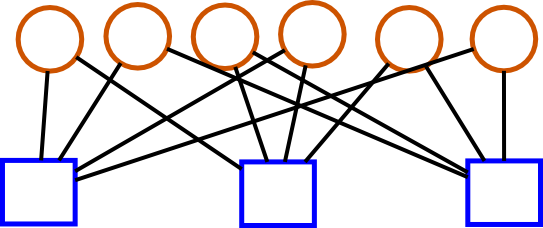
\includegraphics[scale=0.3]{pictures/N6_n2_M3_m4}
\label{fig:ngt16}
 \caption{$m=4$, $M=3$, $N=6$.}
\end{center}
\end{figure}

Clearly this becomes a mess to enumerate systematically. The important point is that the minimum number of switches is higher when $n>1$. This is to be expected since there are more connections per compute node. Compare Fig.~\ref{fig:ngt14},~\ref{fig:ngt16} and Fig.~\ref{fig:fewer_switches_M1},~\ref{fig:fewer_switches_M2}

\begin{figure}[h!]
\begin{center}
\includegraphics[scale=0.3]{pictures/N4_n1_M1_m4}
\label{fig:fewer_switches_M1}
 \caption{$m=4$, $M=1$, $N=4$.}
\end{center}
\end{figure}

\begin{figure}[h!]
\begin{center}
\includegraphics[scale=0.3]{pictures/N6_n1_M2_m4}
\label{fig:fewer_switches_M2}
 \caption{$m=4$, $M=2$, $N=6$.}
\end{center}
\end{figure}



\ \\
As an example using the same parameters as before, when $N=1000$ and $m=24$, the maximum number of switches is now 72,000 (solution 1) and the minimum is greater than the minimum found when $n=1$. The maximum was expected to decrease (compared to the maximum for $n=1$) since there are more ports at the compute node.

\ \\
As a check, the difference between the maximum and minimum number of switches should go to zero as $n$ approaches $N-1$. 

\begin{figure}[h!]
\begin{center}
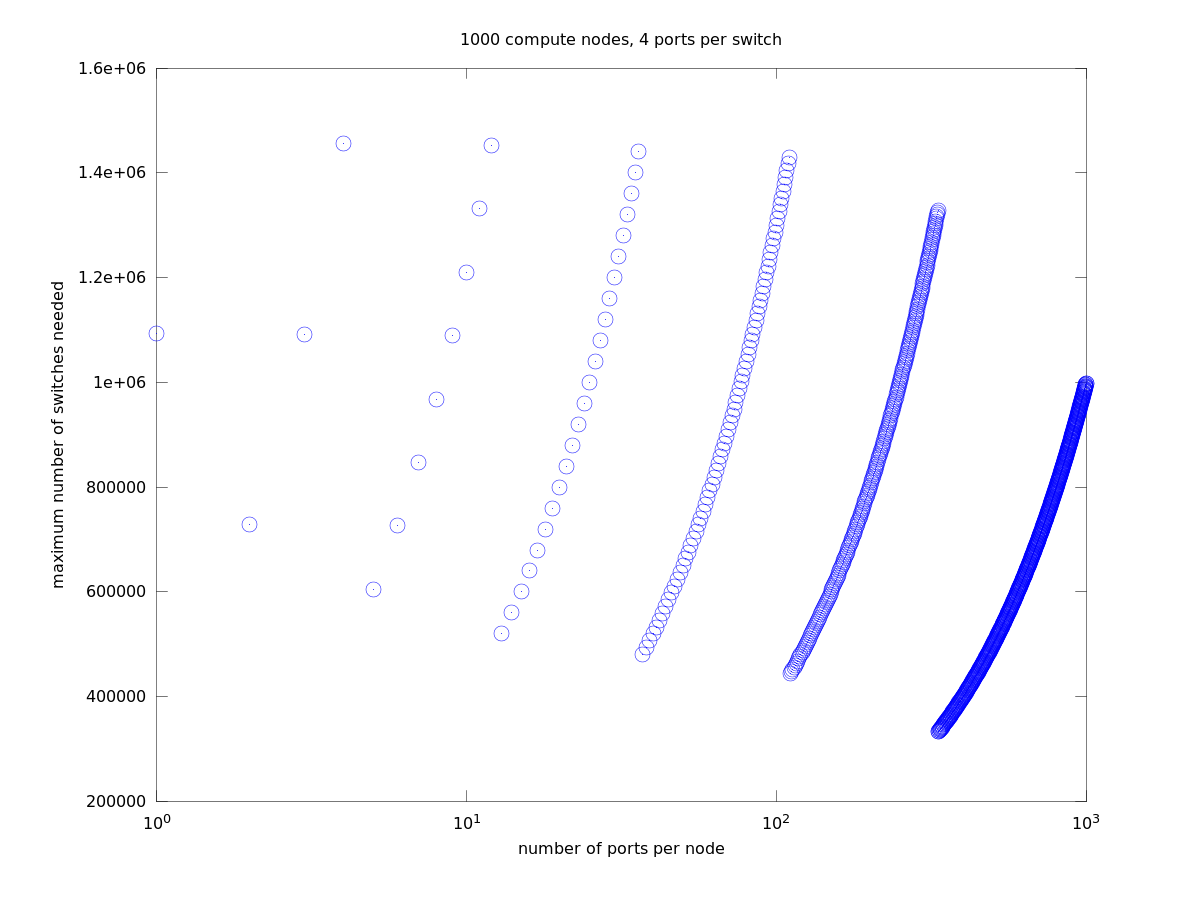
\includegraphics[scale=.3]{pictures/maximum_number_of_switches_needed_versus_compute_node_port_count_for_1000_compute_nodes_and_4_ports_per_switch_semilogx}
\label{fig:max}
 \caption{$m=4$, $M=3$, $N=6$.}
\end{center}
\end{figure}
\begin{verbatim}
 N=1000; m=4; 
 for n=1:(N-1),
   a=1:ceil(log((N-1)./n)./log(m-1));
   M_max(n)=N*n.*sum((m-1).^(a-1));
 end
 n=1:(N-1);
 plot(n,M_max)
 figure; plot(1:N-2,M_max,"o","markersize",15)
 xlabel("number of ports per node"); ylabel("maximum number of switches needed"); title("1000 compute nodes, 4 ports per switch")
 print -dpng maximum_number_of_switches_needed_versus_compute_node_port_count_for_1000_compute_nodes_and_4_ports_per_switch.png
 print -deps maximum_number_of_switches_needed_versus_compute_node_port_count_for_1000_compute_nodes_and_4_ports_per_switch.eps
 figure; semilogx(1:N-2,M_max,"o","markersize",15)
 xlabel("number of ports per node"); ylabel("maximum number of switches needed"); title("1000 compute nodes, 4 ports per switch")
 print -dpng maximum_number_of_switches_needed_versus_compute_node_port_count_for_1000_compute_nodes_and_4_ports_per_switch_semilogx.png
 print -deps maximum_number_of_switches_needed_versus_compute_node_port_count_for_1000_compute_nodes_and_4_ports_per_switch_semilogx.eps
 figure; loglog(1:N-2,M_max,"o","markersize",15)
 xlabel("number of ports per node"); ylabel("maximum number of switches needed"); title("1000 compute nodes, 4 ports per switch")
 print -dpng maximum_number_of_switches_needed_versus_compute_node_port_count_for_1000_compute_nodes_and_4_ports_per_switch_loglog.png
 print -deps maximum_number_of_switches_needed_versus_compute_node_port_count_for_1000_compute_nodes_and_4_ports_per_switch_loglog.eps
\end{verbatim}
 

\section{future task list}

Once the hop counter is implemented, it would be useful to validate metrics against analytic values for mesh, torus, fat tree topologies.


\end{document}
